\documentclass[12pt]{article}
 
% \usepackage{amsmath,amsthm,amssymb}
\usepackage{hyperref}
\usepackage{graphicx}
\usepackage[outer=3.15cm]{geometry}
% \geometry{a4paper, body={6.2in,9in}}
\geometry{a4paper,body={6in,9in}}

\linespread{1.2}

\newenvironment{statement}[2][Statement]{\begin{trivlist}
\item[\hskip \labelsep {\bfseries #1}\hskip \labelsep {\bfseries #2.}]}{\end{trivlist}}
\begin{document}
\title{Mixed Reality Prototyping for Retail: Insights from the Meta/nextReality.Hamburg Hackathon} 
\author{Moritz Friedrich, Karim Djemai}
\maketitle

\begin{abstract}
    This report documents our participation in a hackathon organized by Deutsche Telekom, the University of Hamburg, NextReality.Hamburg eG, and Meta in May 2024. The event challenged participants to create an immersive in-store experience for Deutsche Telekom customers using XR technology, with the goal of improving the waiting experience in retail stores. Our team developed a Mixed Reality (MR) prototype that enabled customers to explore a selection of Telekom’s offerings interactively while waiting in line. Using Unity 3D with Meta's XR MR Utility Kit (UPM), we implemented a mixed reality (MR) experience that featured product-related virtual worlds. Despite challenges related to code structure and tight deadlines, we successfully created a functional prototype and secured a win by jury vote. This report provides an overview of the design process, technical implementation, and potential future improvements, such as enhanced interactivity and accessibility.
\end{abstract}

\section{Introduction}
In May 2024, we became aware of an exciting opportunity to participate in a hackathon organized by Deutsche Telekom, the University of Hamburg, NextReality.Hamburg eG, and Meta. The event was set to take place on the 23rd and 24th of May 2024, with a kick-off meeting held the Friday before, where the topic for the hackathon was revealed. In a following first team meeting the groundwork for the event was laid. 

During the kick-off meeting, the organizers presented the theme of the hackathon: "Creating an immersive in-store experience for Deutsche Telekom customers using XR technology." This concept was built around addressing a common issue faced by many customers — waiting in line at Telekom stores to receive personal support. The challenge was to devise a solution that not only entertained customers during their wait but also provided a useful and interactive way for them to explore Deutsche Telekom’s offerings.

Following the presentation, we participated in a team formation session, where participants could collaborate and brainstorm ideas. Our team came together with a shared interest in tackling this challenge and many ideas were brought up and discarded again until a rough layout of the project was created.

The requirements for our solution were specific: it had to be engaging, intuitive, and self-explanatory. We knew that in order to stand out, our prototype needed to offer a seamless and immersive experience, allowing customers to explore products and services in an interactive environment. With this in mind, we brainstormed various ways to integrate MR technology into the in-store experience, ensuring that it would be accessible to a broad audience, regardless of their prior experience with XR technology.

After two intense days of brainstorming, designing, and coding, we presented our prototype to the jury. Our solution focused on an MR experience that allowed customers to virtually explore a selection of Deutsche Telekom’s products, learn about services, and even receive virtual guidance, all while they waited in the store. 

In the end, our hard work paid off. Our team won the hackathon by a jury vote, which was a thrilling moment for all of us. The victory came with the exciting prize of Meta Quest 3 headsets, a testament to the potential of our solution and the promising future of XR.

In \autoref{sec:process} we describe our individual experience and our processes during the hackathon, \autoref{sec:idea} explains the fundamental ideas underlying our prototype and \autoref{sec:implementation} describes implementation detail for the prototype. In \autoref{sec:problems} we show problems of the prototype and explain what could still be expanded upon in the future and \autoref{sec:discussion} finally discusses the project.


\section{Process}
\label{sec:process}
Our team, composed of three members — Bado Völckers, Karim Djemai, and Moritz Friedrich, all students or former students of Human-Computer Interaction at the University of Hamburg — began brainstorming shortly after the hackathon’s kick-off meeting. Following an initial rough sketch of ideas, we dedicated the week leading up to the event for some preparation.

During this time, task distribution was determined largely by access to resources. Both Karim and Bado had access to the necessary hardware, so they took the lead on laying out the technical foundation. This preparation involved creating the Unity project and integrating all the necessary plugins required to support the MR experience. They also began implementing the base functionality of the prototype, ensuring that we had a solid framework in place for the hackathon itself. To facilitate collaboration, we set up a GitHub repository where the project could be developed and maintained. Due to geographic constraints, Moritz could not physically join them during this preparation period, so communication and coordination took place entirely online. We used digital platforms to ensure all team members were on the same page, sharing progress updates and refining our plan for the hackathon.

When the hackathon officially began on May 23rd, we gathered at the Meta office in Hamburg, the event’s on-site location. The day started at 9 am with a warm welcome from the organizers. After setting up our workstations and attending a brief introduction, we had a chance to fuel up with breakfast before diving into the main task. 

We spent the majority of that first day focused on development, building upon the technical groundwork that had been laid the week before. Our primary goal was to rapidly prototype and test the core functionality of the experience we had envisioned during our preparation phase (see \autoref{sec:idea}). At 1 pm, we paused for lunch, using the break to reflect on our progress and make necessary adjustments to our strategy. Following lunch, we resumed work, continuing to code and refine the experience late into the evening. By 10 pm, we were required to leave the building, but we had made significant progress in creating an interactive, immersive prototype.

The second day of the hackathon, May 24th, began even earlier, with teams arriving at 8 am to resume their projects. With the official deadline set for 1 pm, the pressure to finalize our prototype was high. We worked through the morning, focusing on polishing the experience, troubleshooting any remaining issues, and ensuring the prototype met the hackathon's requirements. By the time the deadline arrived, we had just managed to create a functional prototype that incorporated most of our intended features.

After the hacking period concluded, each team presented their project to the jury. Following a series of brief presentations, three finalist teams were selected. As finalists, we were given the task of preparing a more detailed 10-minute PowerPoint presentation to showcase our prototype. This final presentation was a crucial opportunity to highlight the technical and creative merits of our solution, as well as the ways in which it addressed the specific problem statement posed by the hackathon organizers.

Our team used this final presentation to demonstrate the innovative aspects of our MR prototype, focusing on how it enhanced the waiting experience in Deutsche Telekom stores. We were impressed with all the protoypes presented by fellow participants. 

\section{Idea of the prototype}
\label{sec:idea}
The core concept of our prototype revolves around creating an augmented reality (AR) experience that enhances the in-store environment by showcasing Deutsche Telekom’s products in an immersive and engaging way. The AR world we envisioned is not just a static display of products but an interactive space where users can explore and experience the functionality of the products in a dynamic and captivating manner. By blending the physical space of the store with an AR overlay, we sought to transform the mundane task of waiting into a highly interactive experience.

At the heart of our prototype is a snowglobe-inspired orb that hovers above the various product widgets placed around the user. This orb acts as a visual gateway, displaying miniature versions of different virtual worlds (see \autoref{fig:phone}). Each world is connected to a product widget, and when a user picks up a widget, the AR environment transitions seamlessly into the corresponding world (see \autoref{fig:phone_world}).  The transition is visually compelling - over the span of about one second, the orb appears to expand and envelop the user, transporting them from the store into the orb-world. This immersive transition ensures that the experience feels fluid and natural, helping the user feel more engaged with the products on display. 

\begin{figure}[ht]
    \centering
    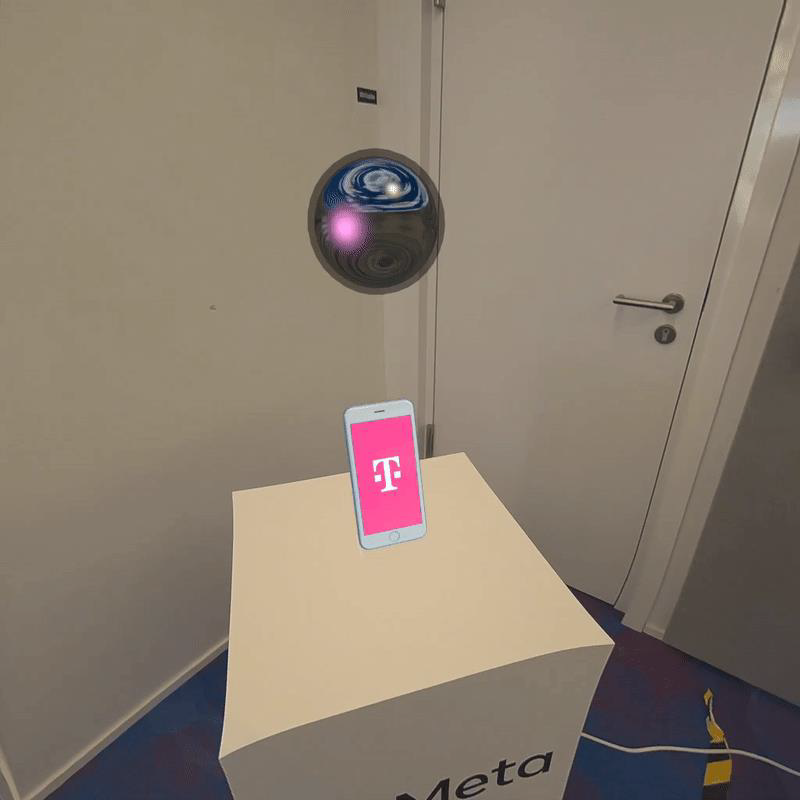
\includegraphics[width=0.5\linewidth]{images/phone.png}
    \caption{The phone widget with its hover orb.}
    \label{fig:phone}
\end{figure}

\begin{figure}[ht]
    \centering
    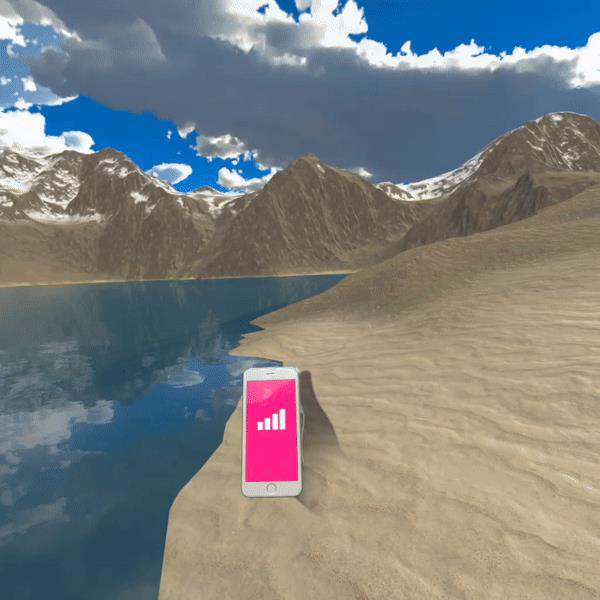
\includegraphics[width=0.5\linewidth]{images/phone_world.png}
    \caption{The virtual world the user gets teleported to, when grabbing the phone widget.}
    \label{fig:phone_world}
\end{figure}

We designed the prototype with three interactive product widgets, each associated with a unique AR world:
\begin{description}
    \item [Smartphone Widget] When the user picks up the smartphone widget, the AR environment morphs into a remote mountain location, where the user is still holding the smartphone and sees an animation showing that there is still full network connectivity. This world serves as a showcase for the connectivity and versatility of telekom's mobile service, illustrating how their products can keep users connected even in the most isolated locations. 

    \item [IP Router Widget] The second widget, an IP router, transports the user to a virtual apartment environment. In this world, users are presented with a minigame where they must plug a cable into the router to restore the apartment's internet connection. As soon as it is connected, two screens in the background start playing videos that have previously been buffering due to the slow connection. This gamified experience not only demonstrates the functionality of Telekom’s routers but also engages users in an interactive task, making the learning process both enjoyable and informative.

    \item [TV Remote Widget] The third widget, a TV remote, creates an entertaining and unexpected experience. When the user picks it up, the virtual TV starts playing a video, and suddenly a football is projected out of the TV into the AR space. This playful interaction emphasizes the immersive potential of Telekom’s media offerings, bringing the entertainment experience beyond the screen and into the physical world around the user.
    
\end{description}

To further enhance the user experience, we introduce a virtual robot agent (see \autoref{fig:robot}. This agent is designed to guide users through the AR environment, explaining how to interact with the products and navigate the virtual worlds. Equipped with text-to-speech functionality, the robot agent ensures that the experience is user-friendly and accessible to a wide range of customers, regardless of their familiarity with AR technology. This agent can be strategically placed within the AR world, providing instructions and information to users in real-time, making the experience as self-explanatory as possible.

\begin{figure}[ht]
    \centering
    \includegraphics[width=0.5\linewidth]{images/robot.png}
    \caption{The text-to-speech robot agent introduces the users to the abilities of the prototype in a user friendly way, regardless of their former experience with MR technology.}
    \label{fig:robot}
\end{figure}

Additionally, the prototype includes a store employee mode, allowing Telekom staff to configure the AR experience by placing the product widgets in the virtual space. This mode enables employees to customize the AR environment based on the store’s layout and the customer’s needs, offering a flexible and adaptable solution for various retail environments.

Overall, the idea behind our prototype was to not only showcase Telekom’s products but to do so in a way that captivates customers, keeps them engaged, and transforms their in-store experience into an interactive journey through multiple virtual worlds. By incorporating familiar elements like smartphones and TV remotes into imaginative MR environments, we aimed to create an experience that is both entertaining and informative, while using advanced MR technology to address the challenge posed by the hackathon.

\section{Implementation}
\label{sec:implementation}
The technical implementation of our prototype was built using Unity 3D. To achieve the MR functionality required for the project, we integrated Meta's XR MR Utility Kit (UPM), which provided the necessary tools and support for developing MR applications. This combination of Unity and the UPM allowed us to efficiently create a seamless MR experience with room scanning, world interaction, and object visualization capabilities.

Given the distributed nature of our team’s preparation, we collaborated through Git, a version control system that allowed multiple members to work on the project simultaneously. Through this cooperative workflow, we were able to push updates, review each other's code, and resolve conflicts in real-time. This setup was essential in keeping development organized, especially as the scope of the project grew during the hackathon.

\subsection{Custom Shader}
One of the standout features of the prototype was the custom shader we developed for the orb visualization. This orb was central to the user experience, serving as the gateway between the physical store environment and the virtual worlds. To make the orb visually compelling, we implemented a shader that created a fake reflection of the virtual world within the orb itself, giving it an otherworldly and immersive quality. This reflection was designed to give users a glimpse of the virtual world they would enter once the orb expanded around them.

Additionally, the shader incorporated a Fresnel effect, which provided a subtle yet striking glow around the edges of the orb. This effect was enhanced with Telekom’s signature magenta coloring. The Fresnel effect made the orb stand out in the inital AR environment, guiding the user’s attention and heightening the sense of immersion as they interacted with the product widgets. The finished orb-shader can be seen in \autoref{fig:phone}.

\subsection{Animations and Room Scanning}
To create smooth and visually appealing transitions within the prototype, we employed tweens for animations. These tweens were used to animate the orb’s expansion as the user picked up a product widget, creating a fluid and organic transition between the physical store environment and the virtual world inside the orb. By using tweens, we were able to control the pacing of the animations with precision, ensuring that the transitions were not only smooth but also engaging for the user. This attention to detail helped maintain the immersive nature of the experience by avoiding jarring or abrupt visual changes.

Another critical component of the prototype’s implementation was the UPM’s room scanning functionality. This feature enabled the AR experience to adapt to the physical layout of the store by scanning the environment and mapping out the available space. Room scanning was essential for accurately placing the product widgets in the AR world and ensuring that the orb-world transitions felt natural and spatially aligned with the real-world environment. The UPM provided us with the tools necessary to dynamically integrate virtual objects into the physical space, enhancing the realism and immersion of the user’s experience.

\section{Problems and Expansion Possibilities}
\label{sec:problems}

As with any rapid development cycle, our hackathon project encountered several challenges, particularly due to the time constraints and the need to deliver a working prototype in just two days. While the core functionality of our MR experience was successfully implemented, there were areas where improvements and extensions could be made, both in terms of technical execution and user experience.

One notable issue was with the robot text-to-speech system, which was designed to guide users through the MR environment by providing verbal instructions. While functional, the system was limited to predefined responses, which made it less dynamic than it could have been. An important extension we identified was to integrate the text-to-speech system with a large language model (LLM)-based chatbot. By doing so, we could create a more interactive and responsive virtual assistant capable of engaging in natural, context-aware conversations with users. This would greatly enhance the user experience, making the robot agent more adaptable and helpful during the in-store interaction.

Another significant issue we faced was the prototyping process itself, which was somewhat unstructured due to the tight deadlines of the hackathon. The codebase developed during the hackathon was, by necessity, produced quickly and often in an ad-hoc manner. This led to unstructured and improvised code, resulting in a number of small bugs that remained unresolved by the end of the event. The code structure lacked the level of organization and modularity that would normally be implemented in a more extended development process. As a result, debugging became more challenging, and certain areas of the prototype — such as the scene transitions — were less polished than we would have liked.

The transition between the real-world environment and the virtual world inside the orb was one of the most visually striking elements of the prototype, but there were still areas where it could be improved. For example, the textures used during the transition could have been of a higher resolution, which would have made the orb expansion effect appear crisper and more realistic. Additionally, the scene loading timing was not perfectly synchronized, which led to a discrete break in transitions. These timing issues could be addressed with a more refined approach to asset loading and optimization, ensuring that the user experiences a smoother and more cohesive transition when moving between the physical and virtual worlds.

From an accessibility standpoint, our prototype also had some limitations. One major issue was the lack of subtitles for users who are deaf or hard of hearing, making it difficult for these users to engage with the robot agent’s spoken instructions. Furthermore, the visual design did not incorporate high-contrast elements, which could make it less accessible to individuals with visual impairments. These oversights highlight the importance of considering accessibility from the outset of the design process, and future iterations of the prototype would need to address these issues to ensure that the MR experience is inclusive for all users.

In terms of extensions, the prototype offers significant potential for further development. One possibility is enabling multiple users to interact within the same MR space simultaneously. This would open up new opportunities for collaborative or competitive experiences, as customers could explore Telekom’s offerings together, interact with shared virtual objects, or even participate in multiplayer mini-games. Another extension could involve showcasing a broader and customizable range of Telekom products. By allowing store employees to easily swap in different virtual products, the MR experience could be tailored to specific stores or customer demographics.

Additionally, integrating LLM-based natural language processing into the virtual assistant would enable users to engage in more sophisticated dialogues with the robot agent. Combining this with speech-to-text and text-to-speech capabilities would create a conversational agent that not only speaks but also listens, significantly enhancing the interactivity of the experience. 

In summary, while our prototype was functional and met the requirements of the hackathon, there were clear areas for improvement in terms of code quality, transition effects, accessibility, and potential extensions. Addressing these challenges and implementing the suggested extensions would greatly enhance the prototype’s functionality, user experience, and overall impact in a real-world retail environment.

\section{Discussion}
\label{sec:discussion}

Participating in the hackathon was an incredibly valuable experience for our team, both in terms of personal growth and professional development. The event highlighted how much can be accomplished in a short time frame when the right combination of pressure, focus, and teamwork is applied. It was remarkable to see how we could start from an initial concept and, within the span of just two days, create a fully functional prototype that integrated advanced technologies like augmented reality and virtual agents. This experience demonstrated the potential of hackathons to push participants beyond their usual limits, encouraging rapid problem-solving and innovation.

The time constraints forced us to make quick decisions and focus on the most critical tasks, and this high-pressure environment helped streamline our workflow. We were able to prioritize the essential components of the project, which resulted in rapid development and significant progress over a short period. However, the speed at which we worked also brought to light the importance of maintaining a balance between speed and structure, especially when it comes to writing clean and well-organized code.

During the event, it was also great to meet fellow hackers from diverse backgrounds. The hackathon created opportunities to network and collaborate, especially during breaks when we could engage in discussions with other participants. These interactions provided new perspectives, as we exchanged ideas, discussed potential challenges, and shared technical insights. Learning about how other teams approached the same problem was both inspiring and educational, offering us a broader understanding of the range of solutions possible within the MR space.

Another highlight of the hackathon was getting an inside look at the Meta office in Hamburg. It was interesting to experience the atmosphere and environment of a leading tech company, and seeing the workspace provided a glimpse into how the company operates on a day-to-day basis. The office’s modern, open layout and advanced facilities were a fitting backdrop for the innovation-driven event, and it was motivating to work in such a cutting-edge space. This insight into the Meta office also contributed to the overall excitement and energy of the hackathon.

Finally, the hackathon left us feeling motivated to continue developing the prototype. While we were proud of what we accomplished within the time constraints, we also recognized the potential for further refinement and expansion of the project. The immersive MR experience we created is just the beginning, and there are many exciting possibilities for adding features, improving the user interface, and making the product more robust. The positive feedback from the jury and the opportunity to explore new technologies have inspired us to continue pushing the prototype forward, potentially transforming it into a more polished and market-ready solution.

In summary, the hackathon provided a unique blend of learning, challenge, and opportunity. It taught us the value of working efficiently under pressure, the importance of code quality, and the excitement of collaborating with like-minded innovators. 

\end{document}